\documentclass[a4paper]{jpconf}
\usepackage{graphicx}
\usepackage{lineno}
\usepackage{hyperref}

\begin{document}
%\linenumbers

\title{Techniques and tools for measuring energy efficiency of scientific software applications}

\author{David Abdurachmanov$^1$, Peter Elmer$^2$, Giulio Eulisse$^3$, Robert Knight$^4$, Tapio Petteri Niemi$^5$, Jukka Nurminen$^6$, Filip Nyback$^6$, Goncalo Marques Pestana$^6$, Zhonghong Ou$^6$}

\address{$^1$ Digital Science and Computing Center, Faculty of Mathematics and Informatics, Vilnius University, Vilnius, Lithuania}
\address{$^2$ Department of Physics, Princeton University, Princeton, NJ 08540, USA}
\address{$^3$ Fermilab, Batavia, IL 60510, USA}
\address{$^4$ Research Computing, Office of Information Technology, Princeton University, Princeton, New Jersey 08540, USA}
\address{$^5$ Helsinki Institute of Physics, PO Box 64, FI-00014, Helsinki, Finland }
\address{$^6$ Aalto University, PO Box 11100, 00076 Aalto, Finland}

\ead{Peter.Elmer@cern.ch}

\begin{abstract}
As both High Performance Computing (HPC) and High Throughput Computing
(HTC) are sensitive to the rise of energy costs, energy-efficiency
has become a primary concern in scientific fields such as High
Energy Physics (HEP). There has been a growing interest in utilizing
low power architectures, such as ARM processors, to replace traditional
Intel x86 architectures. Nevertheless, even though such solutions
have been successfully used in mobile applications with low I/O and
memory demands, it is still unclear if they are suitable and more
energy-efficient in the scientific computing environment. Furthermore,
there is still lack of tools to derive and compare power consumption
for these types of workloads, and eventually to support software
optimizations for energy efficiency.

To that end, we have performed several physical and software-based
measurements of workloads from CERN running on ARM and Intel
architectures, to compare their power consumption and performance.
We leverage several profiling tools to extract different aspects
of the experiments, including hardware usage and software
characteristics. We report the results of these measurements and
the experience gained in developing a set of measurement techniques
and profiling tools to accurately assess the power consumption for
scientific workloads. [Version of~\today]
\end{abstract}

\section{Introduction}

 The most recent scientific applications have to process and store considerable 
volume of data. It is foreseeable that the volume of data will increase 
considerably in the future, as technology and requirements enhance. Thus, energy 
consumption has become a major concern amongst the scientific community. \\
 The Large Hadron Collider (LHC) ~\cite{LHCPAPER} at the European Laboratory for 
Particle Physics (CERN) in Geneva, Switzerland, is one of the scientific
projects which computational requirements are too massive for resources to be
 processed and held in one single infrastructure. Hence, data processing and 
storage 
are distributed across the Worldwide LHC Computing Grid (WLCG) ~\cite{WLHC}, 
which uses resources from 160 computer centers in 35 countries. The access to 
such computational resources have made possible CMS ~\cite{CMSDET} and ATLAS
 ~\cite{ATLAS} experiments to achieve important results, such as the discover of 
the Higgs Boson ~\cite{CMSHIGGS, ATLASHIGGS}. While enabling this and other
discoveries, the WLHC consumes massive amount of computational resources and, 
proportionally, energy. Only CMS experiment used approximately 80,000 to 100,000 
x86-64 cores of capacity in 2012, according to ~\cite{ACAT13ARM, CHEP13ARMPHI}.
In the future, with the improvement of the detector's luminosity, the dataset size
will increase by 2-3 orders of magnitude ~\cite{ACAT13ARM, CHEP13ARMPHI},
presenting even more challenges from the energy consumption point of view. \\

 In order to find and develop better solutions to improve energy efficiency in
High Energy Physics (HEP), it is
 important to understand how energy is used by the HEP systems themselves. There 
are 
few tools and techniques that facilitate researchers to reach that goal. Some of
these tools and techniques are outlined and described in this article.  \\
 As energy efficiency becomes a concern, new
solutions have been considered to develop energy efficient systems. One potential
solution is to replace the traditional Intel x86 architectures by low power
architectures such as ARM. A comparison of the energy efficiency between ARMv7 and 
x86 Intel architecture is conducted in this article. The experiments use CMS 
workloads and rely on the techniques and tools described earlier to perform the
measurements.\\

This article is structured as following. Firstly, we describe where is energy consumed in a HTC system. Secondly, we outline some of the tools and techniques available to measure and monitor energy consumption on HTC systems. Finally, we present the results of a comparison between ARMv7 and Intel Xeon architecture using CMS workloads.


\section{Tools and techniques for energy measurement}

important to know where is energy consumed and what tools and techniques are available to do so

\begin{figure}[ht!]
\centering
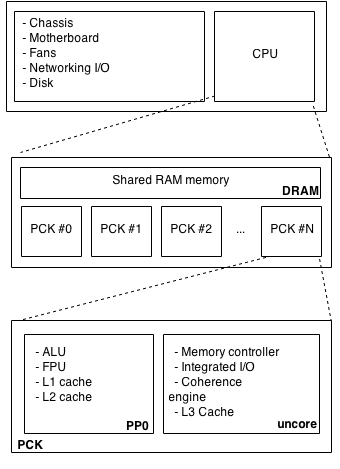
\includegraphics[width=70mm]{img/energy_model.png}
\caption{Components that contribute for power consumption in HPC}
\label{overflow}
\end{figure}

\subsection{External probing devices}

\subsubsection{Noninvasive clamp meters}
\subsubsection{Power distribution units}

\subsection{Internal probing chips}
What is it ? Refer to figure above in order to mention which machine components do the internal probing chips  monitor

\subsubsection{Running Average Power Limit}
Running Average Power Limit (RAPL) provides a platform for monitoring and limiting power of  systems on chip (SoC). It is a Intel's technology which was introduced initially on the Sandy Bridge processors. RAPL platform exposes on-chip measurements via the MSR registers. According to ~\cite{RAPL1}, this technology offers power measurements of the system at a granularity impossible to reach before with other tools.

As documented by Intel in ~\cite{INTELMAN}, there are 3 different domains to sample energy consumed by different SoC components on a server. The domains are: package (accounting for the entire socket), power plane 0 or pp0 (accounting for energy consumed by the core) and dram (sum of energy consumed by memory in a given socket, excluding the core caches). The measurements are dumped in the MSR registers at a frequency of ~1 kHz and are exposed to the user via /dev/cpu/<cpu\_nr>/msr. It is also possible to read and write data from the MSR register using Intel’s open source tool msr-tools ~\cite{MSRTOOLS}. 

In addition to power monitoring of the sockets, it can limit the power consumed by the different domains. This feature, usually referred as power capping, allows the user to define the average power consumption limit of a domain in a defined time window. For more information about RAPL’s features and configurations, refer to section 14.9.1 of Intel’s Developer’s manual ~\cite{INTELMAN}.

- RAPL mode 0 vs RAPL mode 1 \\
"The DRAM RAPL is not enabled in BIOS by default. To enable in BIOS, go to Memory Configuration and change the mode from 'Performance' to 'Power Efficient'. Then select 'Mode 1'. This is the VR (voltage regulator) mode of power estimation. The accuracy of this mode is highly dependent on the OEM platform. For Intel reference platforms the accuracy of DRAM power estimation may produce up to ~30% error"


The advantages of using RAPL for measuring power consumption are a straightforward and already installed tool to perform fine grained measurements of energy consumption on SoC and its components.

On the other hand, the drawbacks are lack of documentation available about the monitoring chip. To the knowledge of the authors, specifications such as error degrees, accuracy and implementation diagrams are not publicly available. In addition, the RAPL technology is vendor locked. Considering those two points, it is difficult to accurately compare and reason power measurements between SoCs from Intel and other vendors.


\subsubsection{TI INA231 and alike}

\subsection{Software based measuring tools}
\subsubsection{powertop and alike}
\subsection{IgProf}
Filip's work \\


\section{Comparison of power efficiency of ARM and Intel}

 \subsection{Workflow and experiments setup}
    Description of the experiments done in ARM ({\it Cortex-A15 Quad and Cortex-A7 Quad 1.4GH}) and Intel ({\it Xeon E5-4650})

\subsection{ARM results}
    Result of measurements done in ARM


\subsection{Intel results}
    Result of measurements done in Intel


\subsection{Analisis}
    Analysis and comparison of above described experiments


\section{Conclusions}

\section*{Acknowledgements}
This work was partially supported by the National Science Foundation, under
Cooperative Agreement PHY-1120138, and by the U.S. Department of Energy.

\section*{References}

\bibliographystyle{unsrt}
\bibliography{acat2014-energy-efficiency}

\end{document}
